
\documentclass[11pt,letterpaper]{article}

% Load some basic packages that are useful to have
% and that should be part of any LaTeX installation.
%
% be able to include figures
\usepackage{graphicx}
% get nice colors
\usepackage{xcolor}

% change default font to Palatino (looks nicer!)
\usepackage[latin1]{inputenc}
\usepackage{mathpazo}
\usepackage[T1]{fontenc}
% load some useful math symbols/fonts
\usepackage{latexsym,amsfonts,amsmath,amssymb}

% comfort package to easily set margins
\usepackage[top=1in, bottom=1in, left=1in, right=1in]{geometry}

% control some spacings
%
% spacing after a paragraph
\setlength{\parskip}{.15cm}
% indentation at the top of a new paragraph
\setlength{\parindent}{0.0cm}


\begin{document}

\begin{center}
\Large
Ay190 -- Worksheet 10\\
Anthony Alvarez\\
Date: February 13, 2014
\end{center}

\section{Simple Boundary-Value Problem}

We will solve the following ODE. 
$$ \frac{d^2y}{dx^2} = 12x - 4, y(0) = 0, y(1) = 0.1$$

First we rewrite the second-order ODE as a system of two first-order ODEs:
$$ \frac{dy}{dx} = u(x)$$ $$ \frac{du}{dx} = 12x -4$$. 

We implement the forward euler integrator as well as the RK2 integrator. We 
can see in ~\ref{fig:converg} that the RK2 integrator comes the closer to 
the true solution $y(x) = 2x^3 - 2x^2 + 0.1x$ than the Euler Integrator, though
they both approximate the solution reasonably well. 

\begin{figure}[bth]
\centering
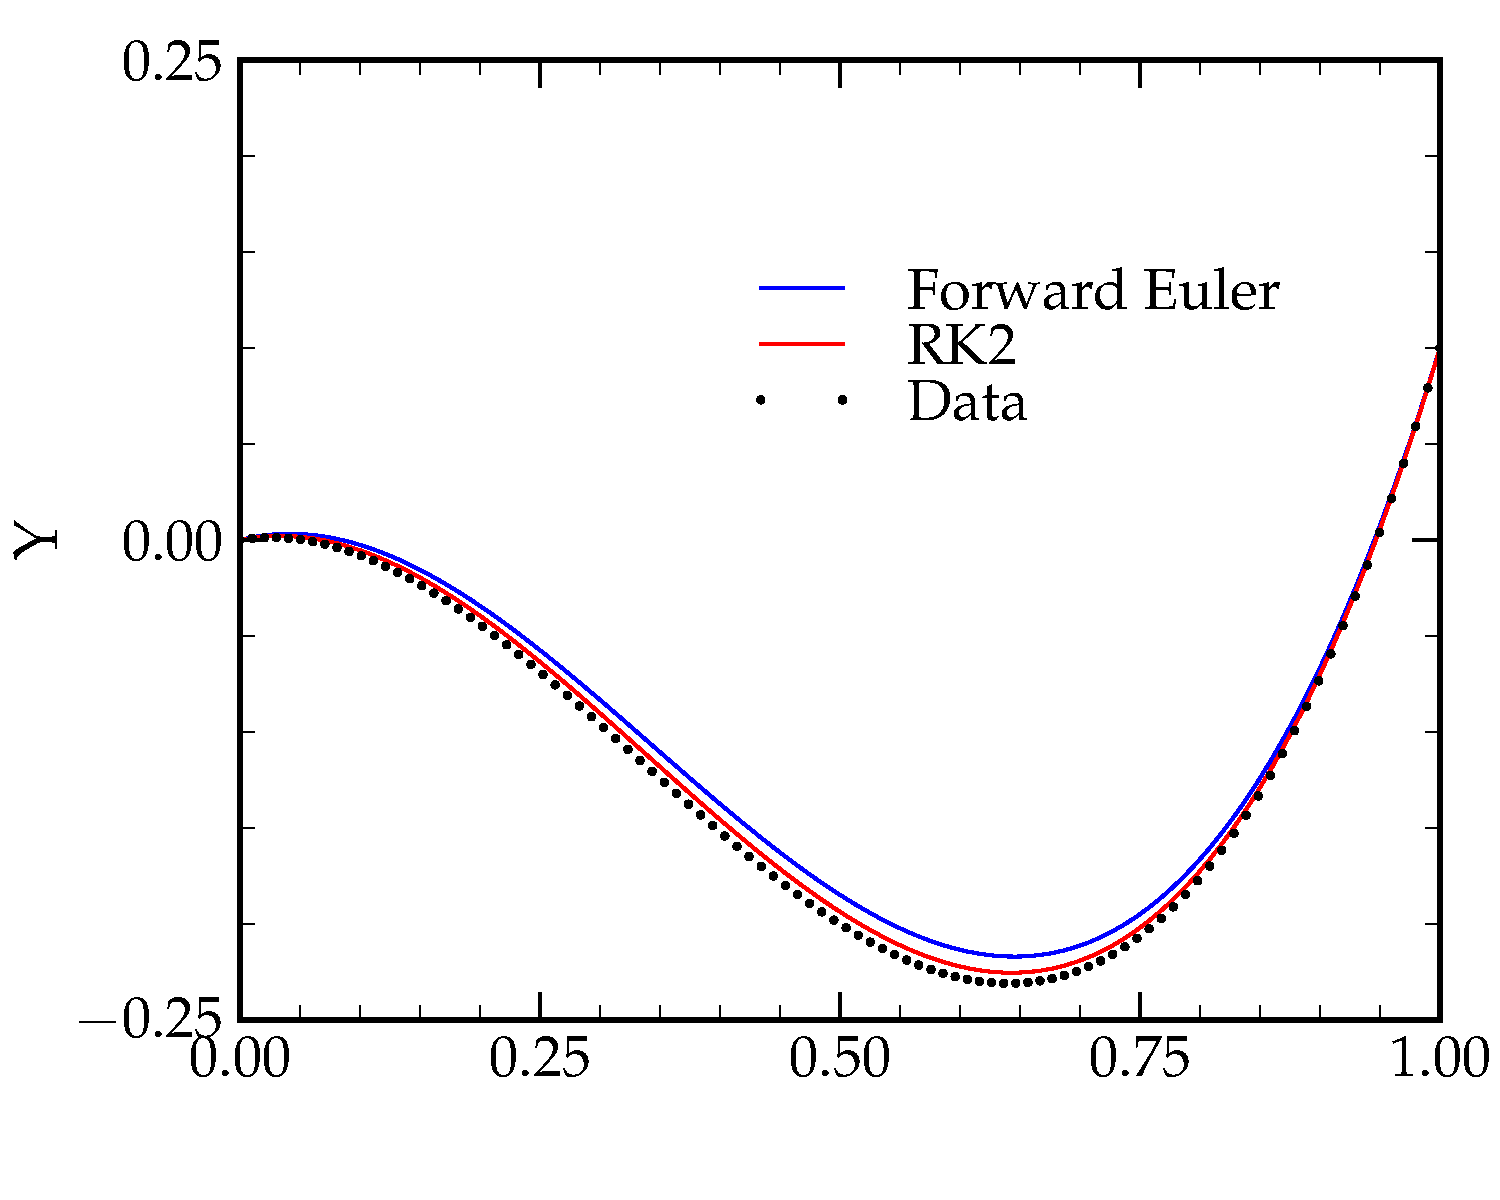
\includegraphics[width=0.5\textwidth]{1.pdf}
\caption{Convergance of Forward Euler and RK2 to the solution $y(x) = 2x^3 - 2x^2 + 0.1x$}
\label{fig:converg}
\end{figure}


\end{document}




